\section{Motivation for Integrating Security requirements into an EDA Flow}
\label{sec:motivation}

%In this section, we provide a concrete example that highlights the fact that existing EDA optimizations indeed have an effect on the security of the device. 
%need for a security-aware EDA flow that optimizes security along with the typical requirements. We take an AES-128 design and synthesize it to generate six different netlists each of which is optimized to meet a different objective such as low power, high performance \& smaller area, low power \& smaller area, and high performance \& low power. % as shown in Table~\ref{tab:design}. 
%The design configurations with their area, delay, and power numbers are shown in Table~\ref{tab:design}. We then analyze the side-channel resistance of each netlist using the Mean Traces to Leak (MTL) metric defined in Section~\ref{}. %The number of power traces needed to guess the key, called mean time for disclosure (MTD), is shown in the fourth column of Table~\ref{tab:design}. A higher MTD value indicates that the attacker needs to collect large number of samples in order to guess the AES key and a smaller MTD value indicates that the device can be easily exploited via the power side-channel.

% \todo[inline]{table 1 hardly makes sense! out of 6 designs on the 3rd one actually serves the purpose.}
\begin{table}[t!]
\scriptsize
\centering

\caption{Impact of design requirements on Area, Power, Delay and the magnitude of TVLA score at the end of 4000 traces for an AES design.  }
\begin{tabular}{|c|c|c|c|c|c|}

\hline

\textbf{\begin{tabular}[c]{@{}c@{}}Design \\ Choices\end{tabular}} & \textbf{Area} & \textbf{\begin{tabular}[c]{@{}c@{}}Delay \\ (ns)\end{tabular}} & \textbf{\begin{tabular}[c]{@{}c@{}}Static\\  Power ($\mu W$)\end{tabular}} & \textbf{TVLA}\\ \hline
I -- Area $\downarrow$ Power $\downarrow$ &       78883        &                  0.48                                              &                            492.4                                  & 11.077                                                                          \\ \hline
II  -- Area $\downarrow$        &        58439       &                 0.48                                               &    602.42             &  11.41                                                                                                            \\ \hline
III -- Area $\downarrow$ Delay $\downarrow$      &       82545        &               0.47                                                 &    513.40               & 8.22  \\ \hline
IV -- Power $\downarrow$ Delay $\downarrow$     &     102256          &             0.47                                                   &               683.41     & 10.65 \\ \hline
V --    Power $\downarrow$ &    79097           &             0.48                                                   &     482.80              &   9.95\\ \hline
VI -- Delay $\downarrow$    &        91822       &        0.32                                                        &     2105.8                  &  13.97       

\\ \hline

\end{tabular}
\label{tab:design}
\end{table}
\begin{figure}[t!]
\centering
  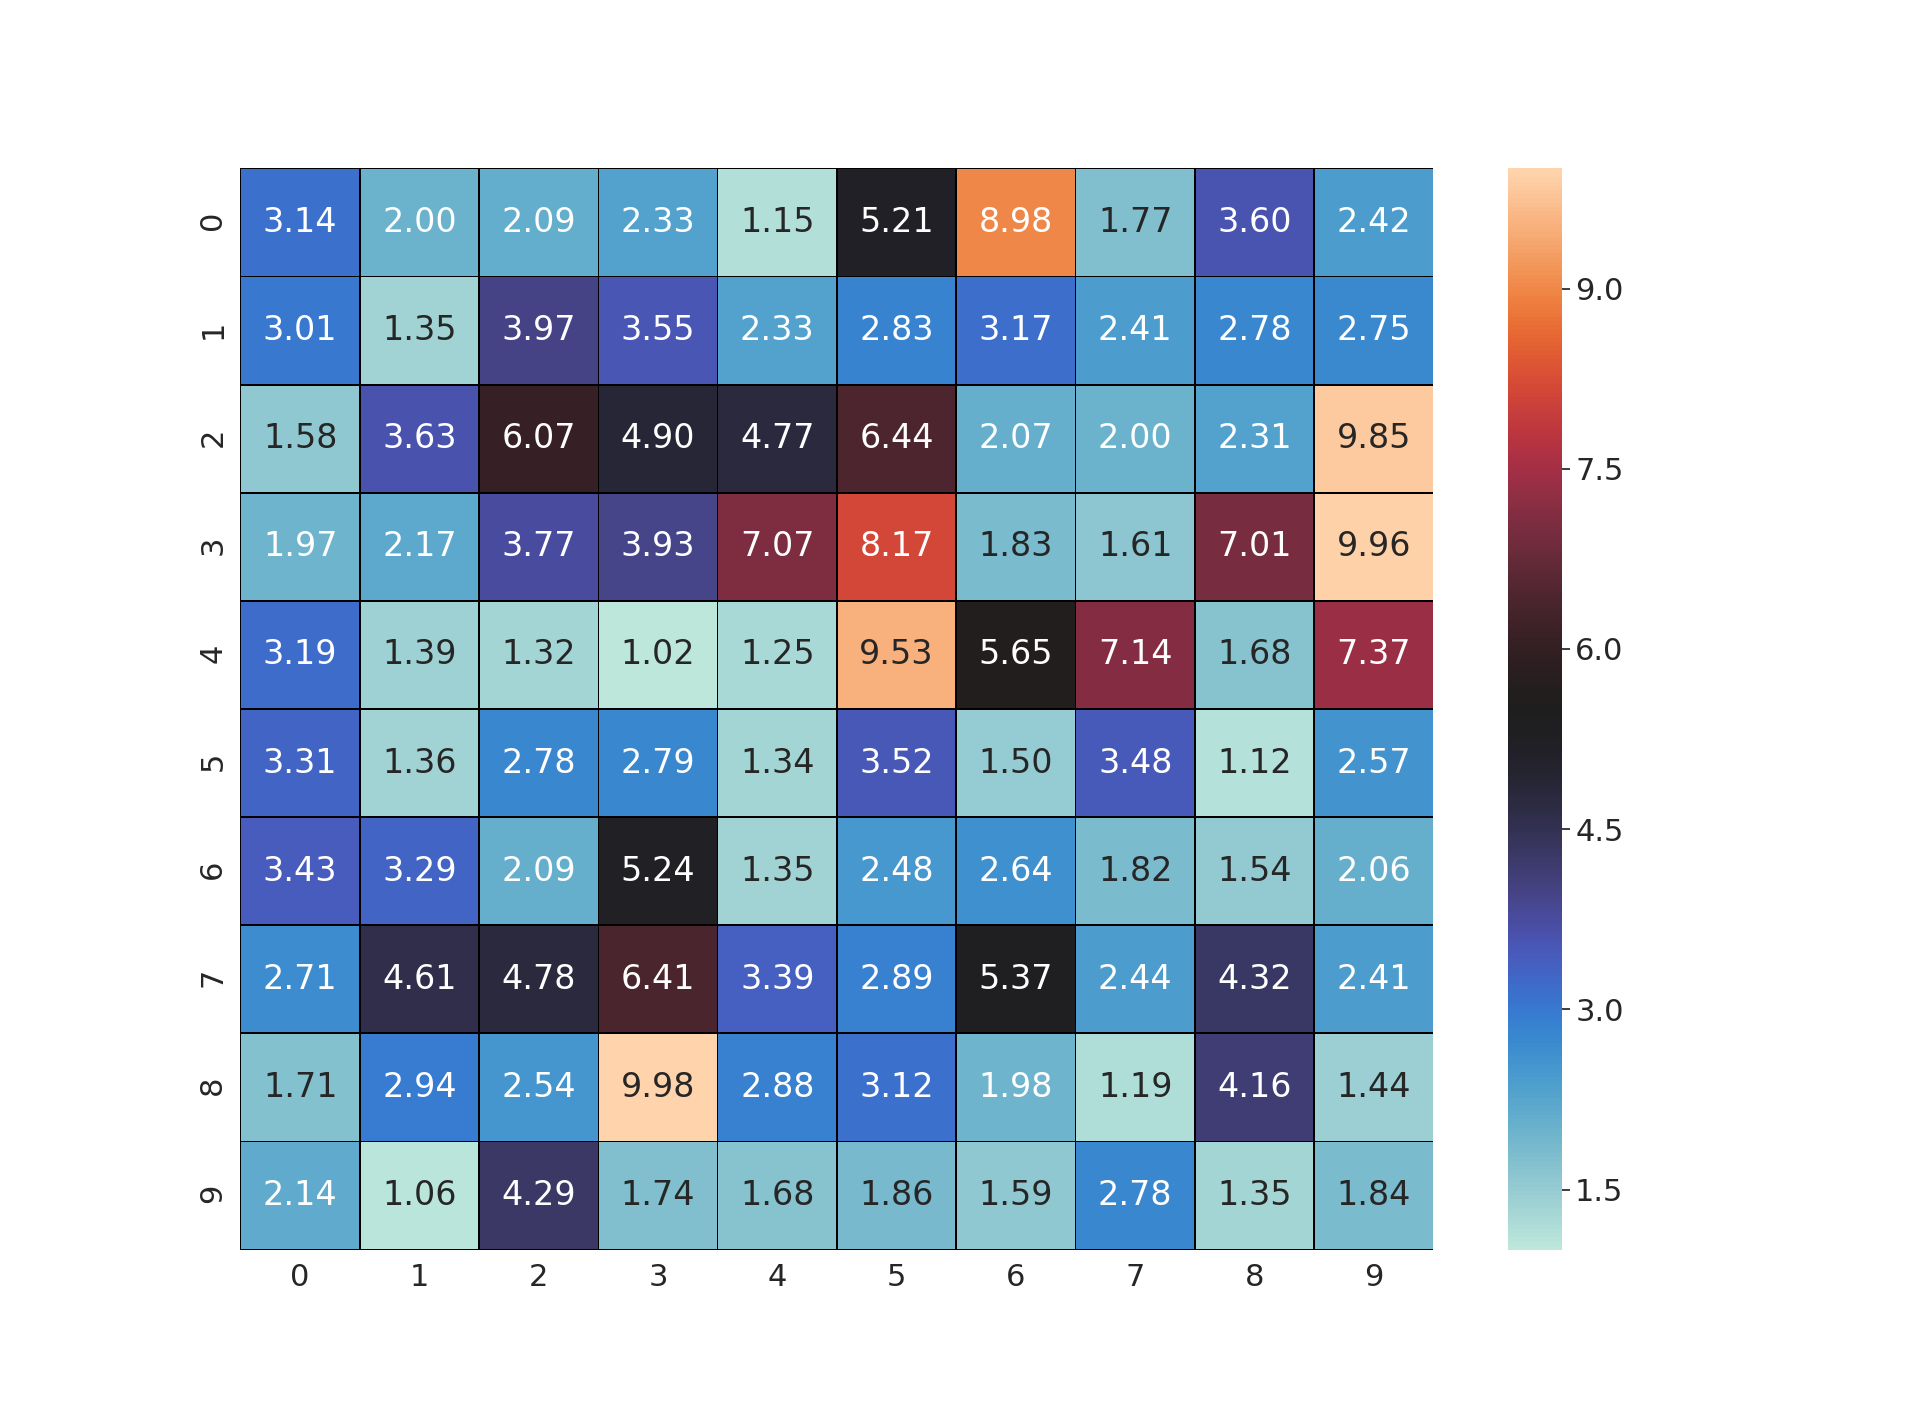
\includegraphics[scale=0.20]{Chapter4/fig/aes_before.png}  
\caption{The TVLA profile of the AES design, with the design divided into a $10\times 10$ grid and the TVLA score of each cell calculated independently. Of the 100 cells, 21 have a TVLA score greater than 4.5. The overall TVLA score of the netlist is 8.22. }
\label{fig:aesopt}
\end{figure}

In this section, we use three critical observations to motivate the use of EDA tools to achieve side-channel security.

\begin{namedthm}{Observation}
EDA algorithms influence the side-channel security of a design.
\end{namedthm}

{\flushleft We} synthesized an AES cipher to meet various design objectives. Table~\ref{tab:design} shows the area, delay, power, and security (TVLA score) of six (I to VI) different netlists. Each netlist was synthesized using the same AES design and used the same EDA tool (Synopsis Design Compiler). The EDA tool was configured with different design requirements for each synthesis. For example, netlist II was synthesized with the objective to reduce area, while netlist IV was synthesized to reduce both power and delay.
For each design, we computed the TVLA score from 4000 pairs of simulated power traces. As seen in the table, we obtain different TVLA scores for each netlist. We thus conclude that design requirements used by an EDA tool have an impact on the overall security of the final device. This experiment corroborates the observations made in~\cite{Verbauwhede:2005, danger:2017, yang:2005}. 
\begin{figure}[t!]
\centering
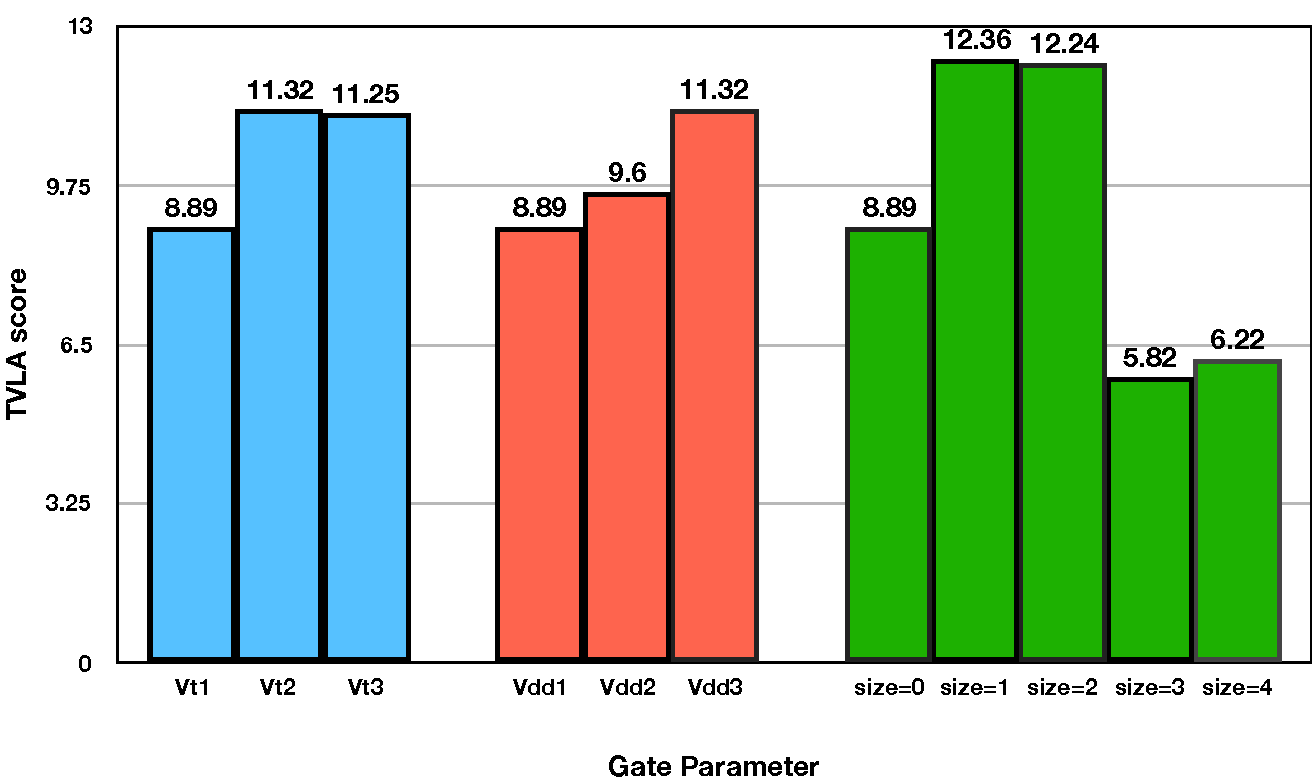
\includegraphics[scale=0.35]{Chapter4/fig/tvla_gate.pdf}
\caption{Variation of TVLA score with $V_{t}$,$V_{dd}$ and $size$ for an AND tree design.}
\label{fig:gateparam}
%\vspace{-15pt}
\end{figure}


% \begin{figure*}[ht!]
% \centering
% \begin{subfigure}{.5\textwidth}
%   \centering
%   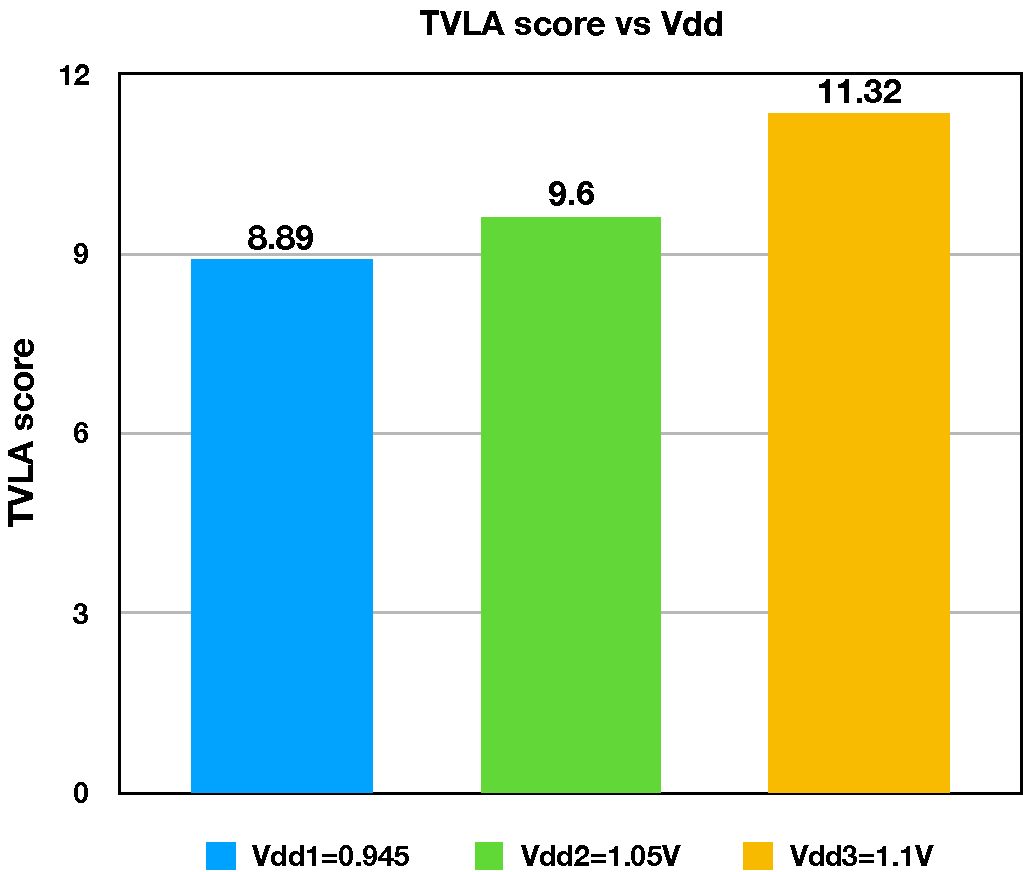
\includegraphics[width=10cm,height=5cm,keepaspectratio]{fig/tvla_vdd.pdf}
%   \caption{Variation of TVLA score with $V_{dd}$.}
%   \label{fig:sub1}
% \end{subfigure}%
% \begin{subfigure}{.55\textwidth}
%   \centering
%   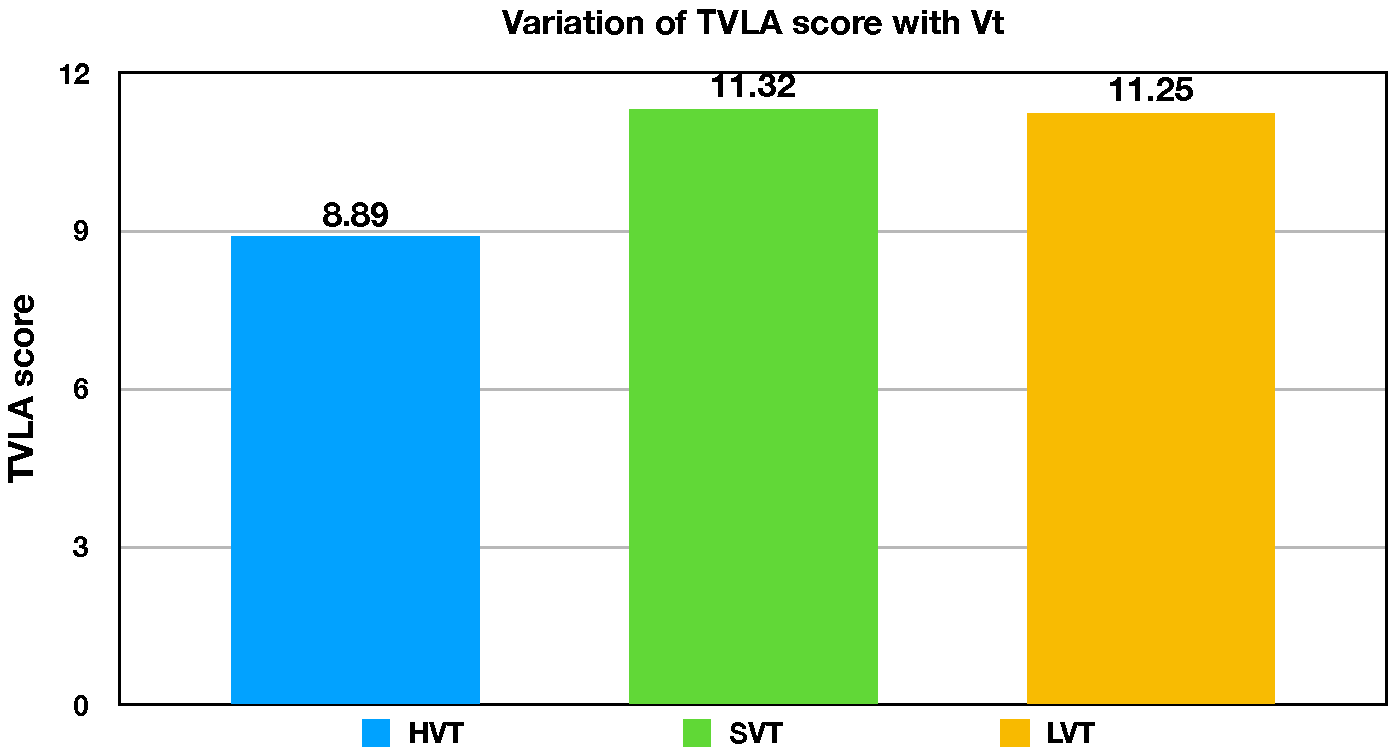
\includegraphics[width=8cm,height=5cm,keepaspectratio]{fig/tvla_vt.pdf}
%   \caption{Variation of TVLA score with $V_{t}$. }
%   \label{fig:sub2}
% \end{subfigure}
% \begin{subfigure}{.75\textwidth}
%   \centering
%   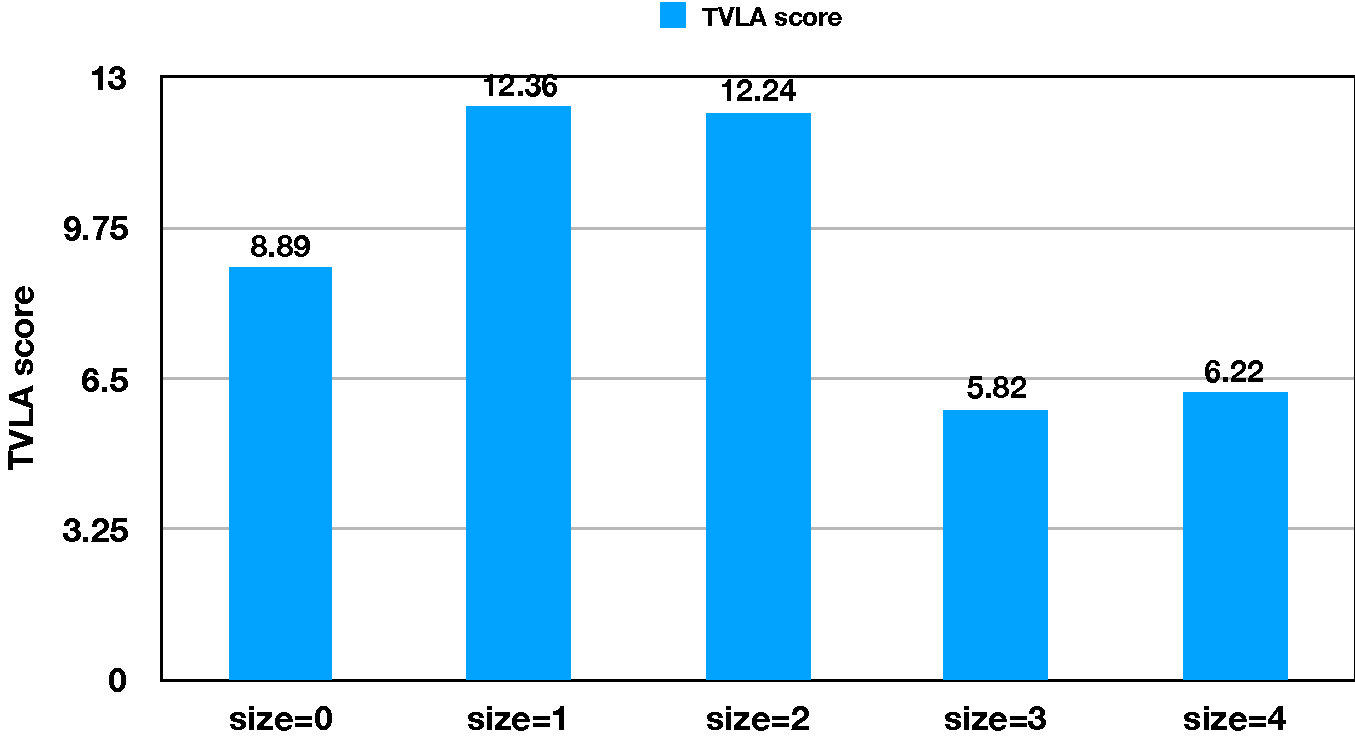
\includegraphics[width=8cm,height=5cm,keepaspectratio]{fig/tvla_size.pdf}
%   \caption{Variation of TVLA score with size. }
%   \label{fig:sub3}
% \end{subfigure}
% % \begin{subfigure}{.75\textwidth}
% %   \centering
% %   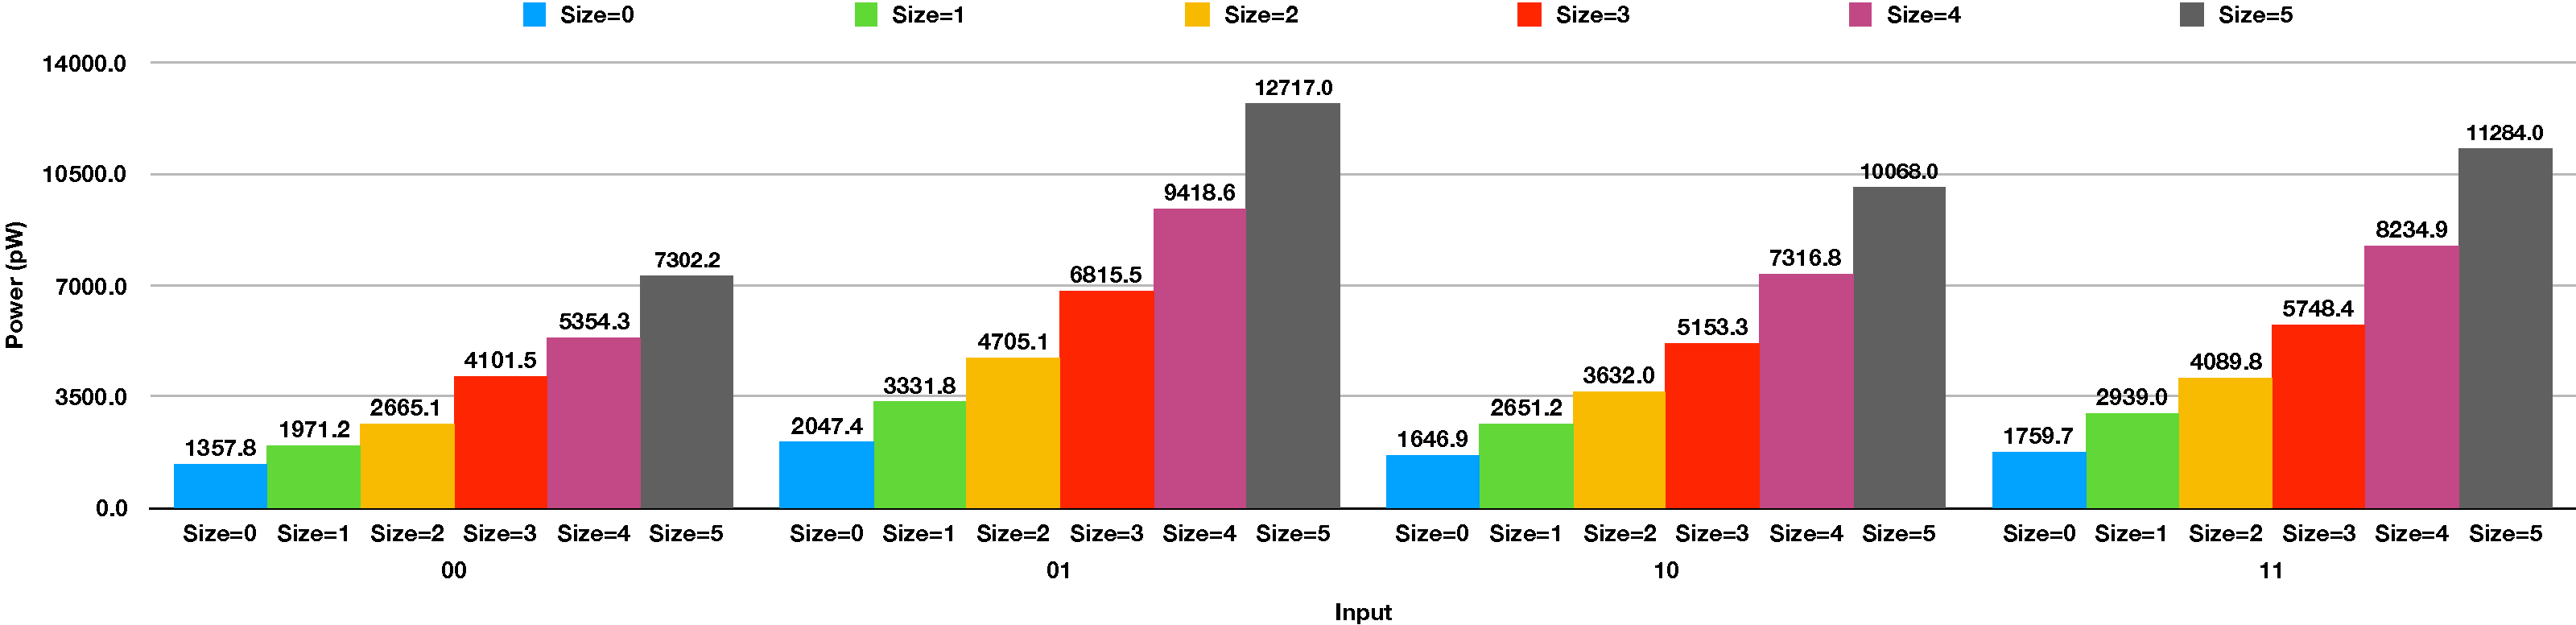
\includegraphics[width=14cm,height=5cm]{fig/sizevsinput.pdf}
% %   \caption{Variation of dynamic power of an AND gate with $size$ and logic level}
% %   \label{fig:sub3}
% % \end{subfigure}%
% % \caption{Figure showing variation of dynamic power of an AND gate with $V_{dd}$, $V_{t}$ and $size$.}
% \label{fig:power}
% \end{figure*}

% \begin{figure*}[ht!]
% \centering
% \begin{subfigure}{.5\textwidth}
%   \centering
%   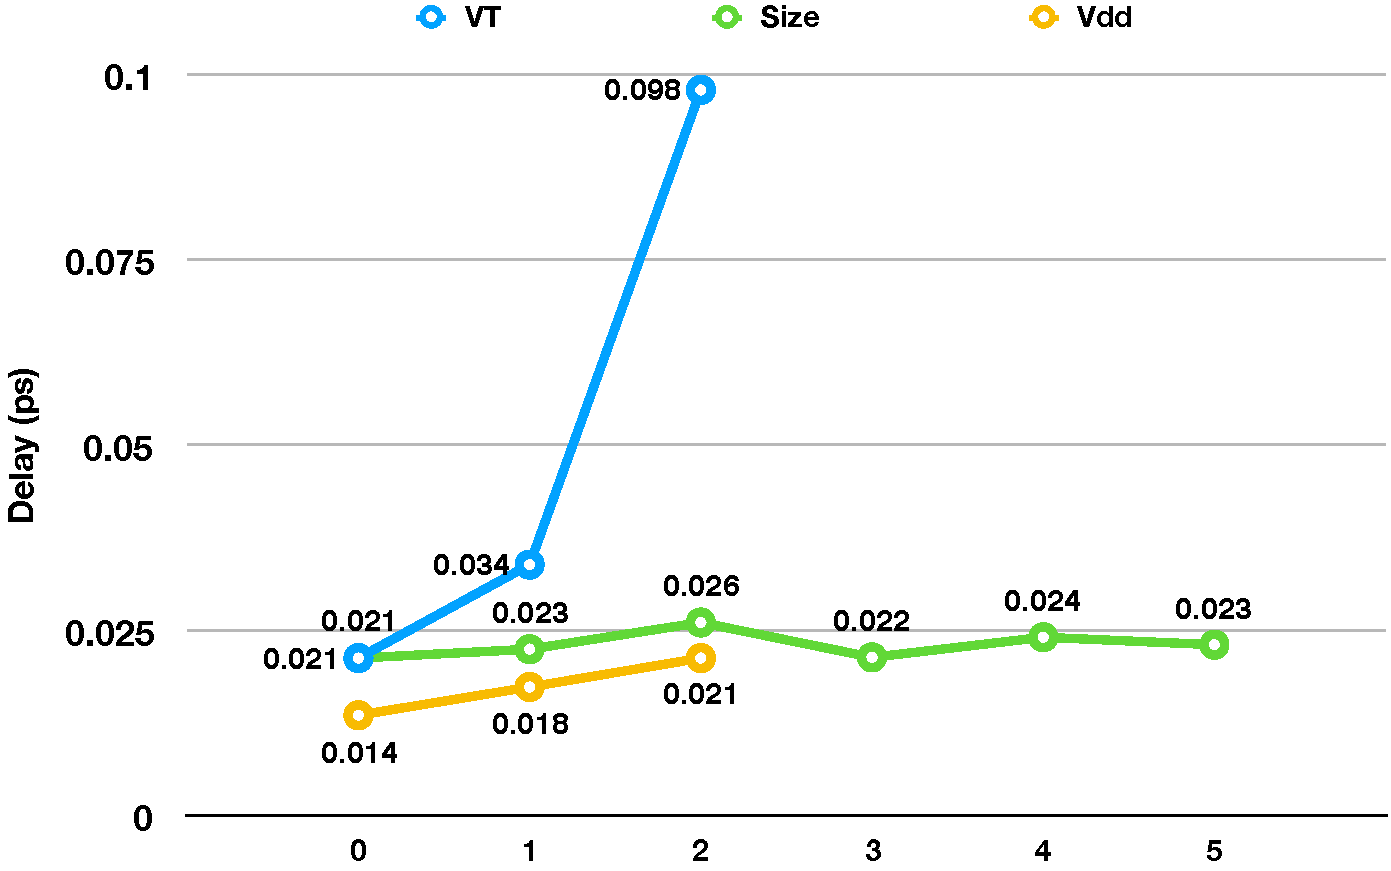
\includegraphics[width=10cm,height=5cm]{fig/delayvariation.pdf}
%   \caption{Variation of delay of an AND gate with $V_{dd}$,$V_{t}$ and $size$.}
%   \label{fig:delay1}
% \end{subfigure}%
% \begin{subfigure}{.55\textwidth}
%   \centering
%   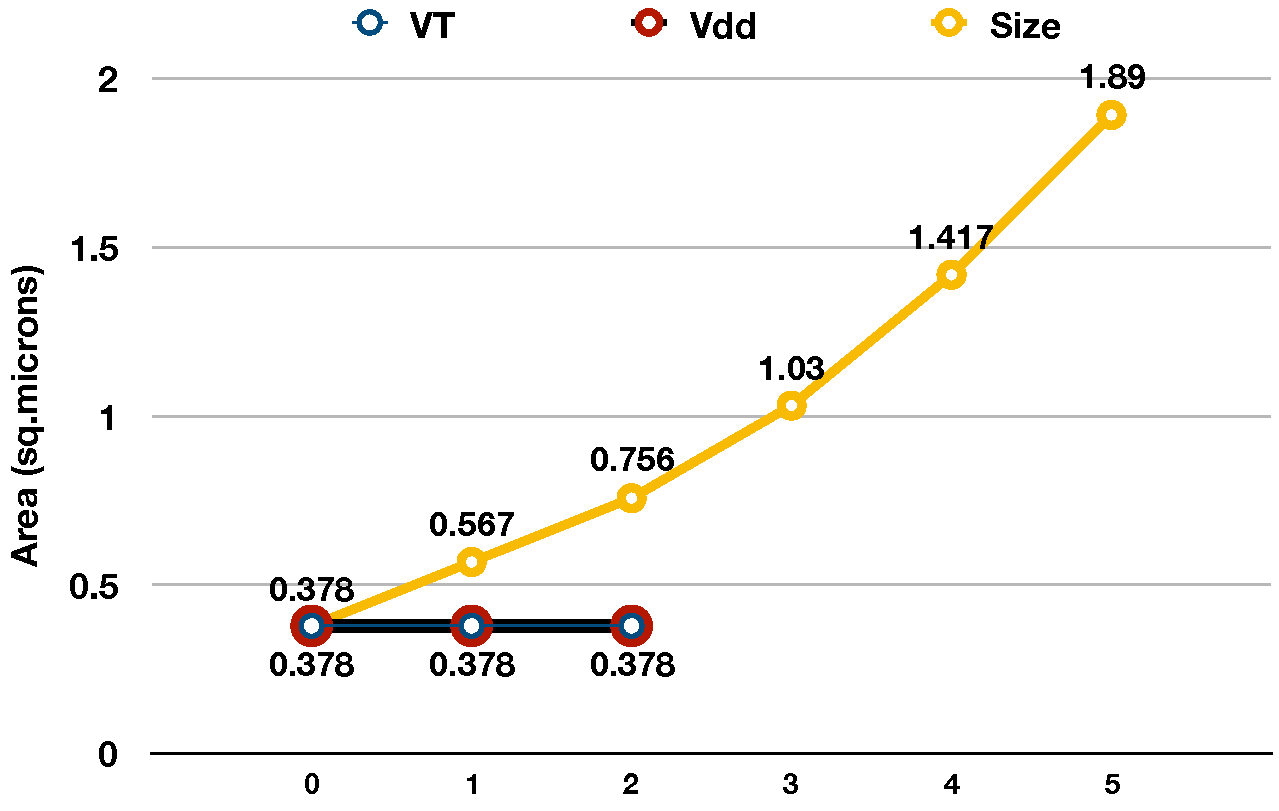
\includegraphics[width=8cm,height=5cm]{fig/areavariation.pdf}
%   \caption{Variation of area of an AND gate with $V_{dd}$, $V_{t}$ and $size$. }
%   \label{fig:delay2}
% \end{subfigure}
% \caption{Figure showing variation of delay and area of an AND with respect to $V_{dd}$, $V_{t}$ and $size$. It can be seen that delay increases with increase in $V_{dd}$, $V_{t}$ and size while area remains constant for $V_{dd}$ and $V_{t}$ scaling and increases with increase in size}
% \label{fig:delay}
% \end{figure*}


\begin{namedthm}{Observation }
Not all regions of the synthesized design contribute equally to the leakage.
\end{namedthm}
{\flushleft There} are certain areas in the design that have a higher leakage compared to other areas. In order to evaluate this, we divided the netlist into a $10 \times 10$ grid and computed the TVLA score for each region independently, thus obtaining 100 different TVLA scores corresponding to various regions in the  netlist. Figure~\ref{fig:aesopt} shows the variations in the TVLA score calculated for netlist III. 
{\sf Karna}, reconfigures the units where leakage is high, so as to reduce the overall side-channel leakage of the design without compromising the other design requirements. 


\begin{namedthm}{Observation }
The side-channel leakage from a gate depends on its  parameters.
\end{namedthm}
In order to observe the impact of each gate configuration on the side-channel leakage, we synthesized an AND-tree design with 16-bit input and 1-bit output, multiple times with different gate configurations. Each synthesis run was done with a different gate configuration. Figure~\ref{fig:gateparam} shows the TVLA scores obtained from 2000 pairs of simulated power traces for each run. It can be seen that changing 
$V_{dd}$, $V_t$ or $size$ options for a gate has an impact on the side-channel leakage of the design.

%Hence, it is important to select gate configurations that meet the design requirements but do not impact the security constraint.
%As mentioned earlier, the EDA tool optimizes the $V_{dd}$, $V_{t}$ and  size of each gate in the design in order to meet a given constraint.We now examine the impact of modifying the design choices by using an AND gate as an example. Figure~\ref{fig:power} shows the variation of dynamic power of an AND gate when the supply voltage $V_{dd}$ and threshold voltage $V_{t}$ are varied. It can be seen that increasing the supply voltage will cause the power consumed by the gate to increase by $\approx5\times-20\times$. We can also observe that the power consumed for different inputs (i.e, $00$, $01$, $10$, and $11$) is different. For example, the difference in the power consumed for inputs $11$ and $01$ at $V_{dd}=1.1V$ is $288$ pW, whereas the difference is $3.5$ pW at $V_{dd}=0.945V$. Such differences can be leveraged to distinguish between the inputs provided at the AND gate and may affect the overall security of the design. A similar observation can be made in figure~\ref{fig:sub2} for $V_{t}$ and figure~\ref{fig:sub3} for varying the gate size. 

A na\"ive approach to achieve security would be to choose gate configurations that provide highest security. However,  na\"ively choosing such gate configurations may violate other design requirements such as delay and power. 
Therefore, there is a need for a careful strategy to vary the gate parameters such that the overall security of the design improves while still meeting the desired design requirements.  
\vspace{-3pt}
% Motivation for post-placement
%It is important to note that the security countermeasures incorporated at any given stage should remain persistent throughout the other stages in the flow. For example, incorporating security at a post-synthesis stage might cause the design to violate area requirements in the placement stage thus requiring re-synthesis. Another consequence is that the tool could optimized out the proposed countermeasures thereby rendering them ineffective. 
%In this work, we therefore choose to introduce the {\sf Karna} module which selects the appropriate gate configuration for each after the design is placed. At this stage, a realistic estimation of the interconnect delay and power density is known. Thus, in this stage, we can accurately gauge the impact of the proposed security based modifications on the area, delay, and performance of the device. 

% a gate $g_{i}$ to be in the critical path of a design iff }




%The problem of securing devices against power side channel attacks has been explored since \cite{} and \cite{}. Techniques like \cite{} and \cite{} have explored software level and device level techniques to address this issue. However, software level techniques only alleviate the symptoms but fail to address the root cause of such vulnerabilities. Device level techniques rely on modifying the physical traits of the device either at gate level as in \cite{}. In this work we explore an alternative idea of mitigating power side-channels at the design level. We motivate the need for such a technique in this section. %This is what disconnected writing gets you, you idiot!

%\indent A power side-channel is said to occur when the device under test consumes drastically different power for a specific input vector than for other random inputs. Mitigating this problem would mean producing a configuration for the device such that it consumes constant or near constant amount of power for any input thereby reducing the statistical variation between the power signature for a fixed input. In device terms this would mean assigning each gate in the device a configuration such that the overall power consumption is fairly constant. 

%\indent In a typical VLSI design flow, the device typically undergoes several optimizations, each with its own objective. The primary of these requirements is performance. The recent power wall and the need for compact devices has led to the emergence of power and area as additional requirements. However, it should be noted that power and area are optimized only if the primary objective is satisfied. 

%\textbf{Observation 1: This drive for a performance optimized design cause the designers to pick gate configurations that, while making the design efficient, might make it compromise the security of the device.}

%It can be seen that while the various algorithms in the EDA flow optimize the design for one or more of performance,area or power, none of them consider the impact on the overall security of the device. This causes the algorithms to pick gate configurations that, while making the design optimal with respect to its requirements, lower the MTD of the device. 





% \indent When we observe the overall power consumption of the device, it can be divided into two components viz. static and dynamic power consumption. Static power is the power that the device consumes during the idle stage and is influenced by temperature, Threshold voltage ($V_t$) and the size of the gate ($g^i_s$). Dynamic power, is the power that is consumed when the device performs some computation, and is affected by the load capacitance ($C_i$), supply voltage $V_(dd)$, and the operating frequency ($F$). It is interesting to see the impact of modifying one or more of these device parameters on the power side-channel of the device.

% \indent Table~\ref{tab2} and~\ref{tab3} shows the leakage power and dynamic power of an inverter. It can be seen that varying $V_t$, $size$, $V_(dd)$ and load capacitance of a gate has an impact on the amount of power that the gate finally consumes. 
% \begin{table}[!ht]
% \begin{tabular}{|c|c|c|c|}
% \hline
% \textbf{Logic Level} & \textbf{$V_{(dd)_1}$} & \textbf{$V_{(dd)_2}$} & \textbf{$V_{(dd)_3}$} \\ \hline
% 00                   &               &               &               \\ \hline
% 01                   &               &               &               \\ \hline
% 10                   &               &               &               \\ \hline
% 11                   &               &               &               \\ \hline
% \end{tabular}
% \label{tab2}
% \caption{Table showing the impact of $V_(dd)$ on the power consumed.}
% \end{table}

% \begin{table}[!ht]
% \begin{tabular}{|c|c|c|c|}
% \hline
% \textbf{Logic Level} & \textbf{$V_{t_1}$} & \textbf{$V_{t_2}$} & \textbf{$V_{t_3}$} \\ \hline
% 00                   &               &               &               \\ \hline
% 01                   &               &               &               \\ \hline
% 10                   &               &               &               \\ \hline
% 11                   &               &               &               \\ \hline
% \end{tabular}
% \label{tab3}
% \caption{Table showing the impact of $V_t$ on the power consumed.}
% \end{table}
% It can be seen that varying $V_t$, $size$, $V_(dd)$ has an impact on the amount of power a gate consumes and thereby it also impacts the power side channel of the entire device. Hence there exists the need for a optimization scheme that takes into account the security of the device. In the next section we introduce Karna, a security aware power optimization scheme.




% %\indent Table~\ref{tab4} shows the various requirements that are addressed during the design manufacturing, it can be noted that security is never viewed as an objective during these stages. This is because quantifying the security or degree of "trust" in a chip is a hard problem to solve in itself. It is harder to quantify the "change" in the degree of trust due to an optimization. Figures~\ref{fig1} and ~\ref{fig2} represent two different optimization choices performed on the same design. It can be seen that 

% %\textbf{Observation 3: There exists a need to reliably quantify the impact of a design optimization on the security of the device.}

% %It can be seen that there exists a need for a design level solution that is able to quantify the impact of design optimizations on security. This will enable designers to explore security aware design optimizations such that performance goals can be achieved while minimizing the vulnerability of the device. In the next section, we will explore how existing metrics can be translated %find a better word
% %into design level requirements and a security aware power minimization scheme. 


